%---------------------------------------------------
% Nombre: capitulo1.tex  
% 
% Texto del capitulo 1
%---------------------------------------------------

\chapter{Planificaci�n}

En este cap�tulo se detallan los enfoques de deep learning usados durante el transcurso de la competici�n as� como la metodolog�a de trabajo y desarrollo llevada a cabo por el equipo durante el transcurso de la pr�ctica para favorecer mejores resultados y sobre todo optimizar tiempos. 

\section{Metodolog�as de Deep Learning}
\label{meto}
Dado que el equipo estaba formado por tres componentes se dividieron las directrices del mismo en las tres vertientes m�s estudiadas dentro de deep-learning:

\begin{enumerate}
\item \textbf{From Scratch}: Esta es la t�cnica que mejores resultados ha ofrecido en la competici�n. Consiste en crear y entrenar una red neuronal desde 0. En casos como el que nos encontramos, tendremos el problema de que hay una muestra muy peque�a de datos para el entrenamiento por lo que habr� que utilizar data augmentation para favorecer su mejora. 
\item \textbf{Transfer Learning}: Esta t�cnica, se basa en utilizar redes ya entrenadas para clasificar un nuevo problema. Si el dominio del problema no es muy diferente a las im�genes usadas para entrenar la red inicial, puede que los resultados sean aceptables y tiempos de entrenamiento nulos si por otro lado, estamos en problemas muy especiales como casos m�dicos esta opci�n no debe ni ser contemplada. En nuestro caso, al ser objetos comunes del mundo real si que la hemos contemplado. 
\item \textbf{Fine Tunning}: Esta t�cnica se basa en la adaptacion de topolog�as muy potentes que son o han sido estado del arte en clasificaci�n de im�genes para un problema en concreto. La idea de esta metodolog�a reside en utilizar las primeras capas de redes ya entrenadas las cuales almacenan datos de curvas y aristas en gran medida y tras ello, se entrenan las ultimas capas con las im�genes de nuestro problema tras lo cual los resultados ser�n bastante buenos o aceptables. 
\end{enumerate}

\section{Planificaci�n temporal}

El proyecto ha sido planificado temporalmente acorde a los siguientes puntos, tareas u objetivos:

\begin{itemize}

\item \textbf{Pruebas con modelos individuales}: En los primeros d�as cada uno de los miembros del equipo estudi� una de las metodolog�as vistas en el punto \ref{meto}. Se hicieron las primeras subidas a Kaggle.  
\item \textbf{Preprocesado}: Una vez se dio con la metodolog�a a seguir, fine tunning, se estudiaron y variaron ciertas variantes del pre-procesado para obtener mejores resultados. 
\item \textbf{Estudio de mejores modelos}: Se estudio el estado del arte en la materia para adaptar al proceso de fine tunning modelos cuya potencia estuviera ya constatada. 
\item \textbf{Reuniones de grupo}: Reuniones de puesta en com�n de resultados y debate de t�cnicas y v�as de estudio. 
\item \textbf{Redacci�n}: Tras la finalizaci�n de la competici�n se abre un per�odo de redacci�n del presente documento. 
\end{itemize}

En la figura \ref{planificacion}, puede verse un croquis sobre el calendario del mes de marzo, en el que se detallan las distintas tareas que se han detallado en puntos anteriores.

\begin{figure}[H]
\centering
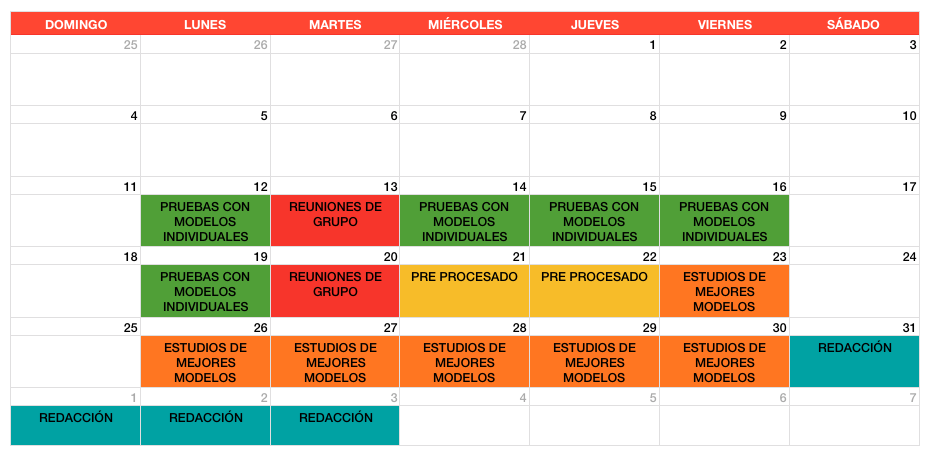
\includegraphics[width=12cm]{./Planificacion/imagenes/plani.png}
\caption{Croquis de la planificaci�n seguida.}
\label{planificacion}
\end{figure} 

\section{Desarrollo}

Para el desarrollo del c�digo se ha usado un repositorio para el control de versiones en GitHub que puede verse en \cite{github}. En este hemos creado ramas para cada uno de los miembros del equipo que eran fusionadas al realizar alg�n avance.

Dado que el proceso de entrenamiento con Keras permite guardar pesos, se ha llevado a cabo un desarrollo basado en \textbf{soluciones intermedias}. Con este m�todo, se guardan los pesos de ciertas redes por lo que otros miembros del equipo por medio del m�todo \textbf{read model} pueden leer estos pesos y utilizarlos para sus experimentos sin necesidad de volver a entrenar modelos ya entrenados. 
\clearpage
%---------------------------------------------------